% Created 2018-06-27 on 12:32
% Intended LaTeX compiler: pdflatex
\documentclass{article}

%%%% settings when exporting code %%%% 

\usepackage{listings}
\lstset{
backgroundcolor=\color{white},
basewidth={0.5em,0.4em},
basicstyle=\ttfamily\small,
breakatwhitespace=false,
breaklines=true,
columns=fullflexible,
commentstyle=\color[rgb]{0.5,0,0.5},
frame=single,
keepspaces=true,
keywordstyle=\color{black},
literate={~}{$\sim$}{1},
numbers=left,
numbersep=10pt,
numberstyle=\ttfamily\tiny\color{gray},
showspaces=false,
showstringspaces=false,
stepnumber=1,
stringstyle=\color[rgb]{0,.5,0},
tabsize=4,
xleftmargin=.23in,
emph={anova,apply,class,coef,colnames,colNames,colSums,dim,dcast,for,ggplot,head,if,ifelse,is.na,lapply,list.files,library,logLik,melt,plot,require,rowSums,sapply,setcolorder,setkey,str,summary,tapply},
emphstyle=\color{blue}
}

%%%% packages %%%%%

\usepackage[utf8]{inputenc}
\usepackage[T1]{fontenc}
\usepackage{lmodern}
\usepackage{textcomp}
\usepackage{color}
\usepackage{enumerate}
\usepackage{graphicx}
\usepackage{grffile}
\usepackage{wrapfig}
\usepackage{capt-of}
\usepackage{caption}
\usepackage{rotating}
\usepackage{longtable}
\usepackage{multirow}
\usepackage{multicol}
\usepackage{changes}
\usepackage{pdflscape}
\usepackage{geometry}
\usepackage[normalem]{ulem}
\usepackage{amssymb}
\usepackage{amsmath}
\usepackage{amsfonts}
\usepackage{dsfont}
\usepackage{textcomp}
\usepackage{array}
\usepackage{ifthen}
\usepackage{hyperref}
\usepackage{natbib}
\RequirePackage{fancyvrb}
\DefineVerbatimEnvironment{verbatim}{Verbatim}{fontsize=\small,formatcom = {\color[rgb]{0.5,0,0}}}
\RequirePackage{colortbl} % arrayrulecolor to mix colors
\RequirePackage{setspace} % to modify the space between lines - incompatible with footnote in beamer
\usepackage{authblk} % enable several affiliations (clash with beamer)
\RequirePackage{epstopdf} % to be able to convert .eps to .pdf image files
\newcommand\model{\mathcal{M}}
\RequirePackage{amsmath}
\RequirePackage{algorithm}
\RequirePackage[noend]{algpseudocode}
\RequirePackage{ifthen}
\RequirePackage{xspace} % space for newcommand macro
\RequirePackage{xifthen}
\RequirePackage{xargs}
\RequirePackage{dsfont}
\RequirePackage{amsmath,stmaryrd,graphicx}
\RequirePackage{prodint} % product integral symbol (\PRODI)
\RequirePackage{amsthm}
\newtheorem{theorem}{Theorem}
\newtheorem{lemma}[theorem]{Lemma}
\newcommand\defOperator[7]{%
\ifthenelse{\isempty{#2}}{
\ifthenelse{\isempty{#1}}{#7{#3}#4}{#7{#3}#4 \left#5 #1 \right#6}
}{
\ifthenelse{\isempty{#1}}{#7{#3}#4_{#2}}{#7{#3}#4_{#1}\left#5 #2 \right#6}
}
}
\newcommand\defUOperator[5]{%
\ifthenelse{\isempty{#1}}{
#5\left#3 #2 \right#4
}{
\ifthenelse{\isempty{#2}}{\underset{#1}{\operatornamewithlimits{#5}}}{
\underset{#1}{\operatornamewithlimits{#5}}\left#3 #2 \right#4}
}
}
\newcommand{\defBoldVar}[2]{
\ifthenelse{\equal{#2}{T}}{\boldsymbol{#1}}{\mathbf{#1}}
}
\newcommandx\Cov[2][1=,2=]{\defOperator{#1}{#2}{C}{ov}{\lbrack}{\rbrack}{\mathbb}}
\newcommandx\Esp[2][1=,2=]{\defOperator{#1}{#2}{E}{}{\lbrack}{\rbrack}{\mathbb}}
\newcommandx\Prob[2][1=,2=]{\defOperator{#1}{#2}{P}{}{\lbrack}{\rbrack}{\mathbb}}
\newcommandx\Qrob[2][1=,2=]{\defOperator{#1}{#2}{Q}{}{\lbrack}{\rbrack}{\mathbb}}
\newcommandx\Var[2][1=,2=]{\defOperator{#1}{#2}{V}{ar}{\lbrack}{\rbrack}{\mathbb}}
\newcommandx\Binom[2][1=,2=]{\defOperator{#1}{#2}{B}{}{(}{)}{\mathcal}}
\newcommandx\Gaus[2][1=,2=]{\defOperator{#1}{#2}{N}{}{(}{)}{\mathcal}}
\newcommandx\Wishart[2][1=,2=]{\defOperator{#1}{#2}{W}{ishart}{(}{)}{\mathcal}}
\newcommandx\Likelihood[2][1=,2=]{\defOperator{#1}{#2}{L}{}{(}{)}{\mathcal}}
\newcommandx\Information[2][1=,2=]{\defOperator{#1}{#2}{I}{}{(}{)}{\mathcal}}
\newcommandx\Score[2][1=,2=]{\defOperator{#1}{#2}{S}{}{(}{)}{\mathcal}}
\newcommandx\Vois[2][1=,2=]{\defOperator{#1}{#2}{V}{}{(}{)}{\mathcal}}
\newcommandx\IF[2][1=,2=]{\defOperator{#1}{#2}{IF}{}{(}{)}{\mathcal}}
\newcommandx\Ind[1][1=]{\defOperator{}{#1}{1}{}{(}{)}{\mathds}}
\newcommandx\Max[2][1=,2=]{\defUOperator{#1}{#2}{(}{)}{min}}
\newcommandx\Min[2][1=,2=]{\defUOperator{#1}{#2}{(}{)}{max}}
\newcommandx\argMax[2][1=,2=]{\defUOperator{#1}{#2}{(}{)}{argmax}}
\newcommandx\argMin[2][1=,2=]{\defUOperator{#1}{#2}{(}{)}{argmin}}
\newcommandx\cvD[2][1=D,2=n \rightarrow \infty]{\xrightarrow[#2]{#1}}
\newcommandx\Hypothesis[2][1=,2=]{
\ifthenelse{\isempty{#1}}{
\mathcal{H}
}{
\ifthenelse{\isempty{#2}}{
\mathcal{H}_{#1}
}{
\mathcal{H}^{(#2)}_{#1}
}
}
}
\newcommandx\dpartial[4][1=,2=,3=,4=\partial]{
\ifthenelse{\isempty{#3}}{
\frac{#4 #1}{#4 #2}
}{
\left.\frac{#4 #1}{#4 #2}\right\rvert_{#3}
}
}
\newcommandx\dTpartial[3][1=,2=,3=]{\dpartial[#1][#2][#3][d]}
\newcommandx\ddpartial[3][1=,2=,3=]{
\ifthenelse{\isempty{#3}}{
\frac{\partial^{2} #1}{\left( \partial #2\right)^2}
}{
\frac{\partial^2 #1}{\partial #2\partial #3}
}
}
\newcommand\Real{\mathbb{R}}
\newcommand\Rational{\mathbb{Q}}
\newcommand\Natural{\mathbb{N}}
\newcommand\trans[1]{{#1}^\intercal}%\newcommand\trans[1]{{\vphantom{#1}}^\top{#1}}
\newcommand{\independent}{\mathrel{\text{\scalebox{1.5}{$\perp\mkern-10mu\perp$}}}}
\newcommand\half{\frac{1}{2}}
\newcommand\normMax[1]{\left|\left|#1\right|\right|_{max}}
\newcommand\normTwo[1]{\left|\left|#1\right|\right|_{2}}
\author{Brice Ozenne}
\date{\today}
\title{Assessing the effect of an exposure on multiple outcomes (with R code)}
\hypersetup{
 colorlinks=true,
 citecolor=[rgb]{0,0.5,0},
 urlcolor=[rgb]{0,0,0.5},
 linkcolor=[rgb]{0,0,0.5},
 pdfauthor={Brice Ozenne},
 pdftitle={Assessing the effect of an exposure on multiple outcomes (with R code)},
 pdfkeywords={},
 pdfsubject={},
 pdfcreator={Emacs 25.2.1 (Org mode 9.0.4)},
 pdflang={English}
 }
\begin{document}

\maketitle

\section*{Abstract}
\label{sec:org1657a8b}
We propose two strategies to assess the relationship between an
exposure (e.g. a disease, a genetic factor) and a set of outcomes
(e.g. a set of psychological outcomes or the binding potential
measured in several brain regions) while accounting for possible risk
factors and confounders. The outcomes can be continuous, categorical,
or a mixture of the two but their number should be smaller than the
number of observations (low-dimensional setting). This document
intends to give a basic understanding of the two strategies, their
limitations, and how to implement them. \textcolor{red}{For
now, only the "multiple univariate regressions" is presented in this
document.} In particular we don't claim that the proposed strategies
give valid or optimal results in every application (they probably do
not). Many other approaches exists (e.g. MANOVA) but won't be
discussed here.

\bigskip

\textbf{Strategies}: 
\begin{itemize}
\item \emph{Multiple univariate regressions}: for each outcome we use a
separate model to model its relationship to the exposure. An
adjustment for multiple comparisons is used for drawing inference.
\item \emph{Joint model}: we model the relationship between the outcomes and
the exposure in a single model. A single test can be used to test
whether there is an association between the exposure and any of the
outcomes.
\end{itemize}
By explicitly modeling the correlation between the outcomes, the
"joint model" strategy, when valid, will provide more powerful tests
compared to the "multiple univariate regressions" strategy. Another
benefit of the "joint model" strategy is the use of latent variables
that may reflect unmeasured biological mechanisms and therefore help
the interpretation of the results. There are however drawbacks with
this approach: it relies on more assumptions and a more complex
statistical modeling. 

\bigskip

\textbf{Inference}: The two strategies enable to quantify the association
between the exposure and the outcomes and to test hypotheses such as:
\begin{itemize}
\item there no association between the exposure and the outcomes. When
rejected, it can further test for which outcomes there is evidence for an
association while adjusting for multiple comparisons in an efficient
way.
\item the association between the exposure and the outcomes is the same for all outcomes.
\end{itemize}
An adjustment is proposed in small sample sizes (e.g. n<100) to
improve the control of the type 1 error rate. This adjustment
has been shown to beneficial in several settings (using simulation
studies) but does not always perfectly control the type 1 error
rate. It is advised to check that validity of the adjustment when
using very small samples or models with many parameters. Resampling
methods (permutation or bootstrap \citep{carpenter2000bootstrap}) may be
preferable in some settings.

\bigskip

\textbf{Diagnostics}: The proposed strategies uses on parametric models that
rely on a set of assumptions. The violation of some of the assumptions
can be tested using the observed data (often with limited
power). Tools to test these assumptions are presented.

\bigskip

\textbf{Software}: we advise to use the R software to implement these
strategies. It can be downloaded at \url{https://cloud.r-project.org/}. R
studio provide a convenient user interface that can be downloaded at
\url{https://www.rstudio.com/products/rstudio/}.  The R code used to carry
out the two strategies will be display in boxes:
\lstset{language=r,label= ,caption= ,captionpos=b,numbers=none}
\begin{lstlisting}
1+1 ## comment about the code
\end{lstlisting}

\begin{verbatim}
[1] 2
\end{verbatim}

while the R output will be displayed in dark red below the box. 


\bigskip

We also recommend the following packages:
\begin{itemize}
\item \emph{data.table}: for data management. See
\url{https://cran.r-project.org/web/packages/data.table/vignettes/datatable-intro.html}
for an introduction and
\url{https://github.com/Rdatatable/data.table/wiki} for more
documentation.  A synthetic description of the functionalities can
be found at
\url{https://s3.amazonaws.com/assets.datacamp.com/img/blog/data+table+cheat+sheet.pdf}
\item \emph{ggplot2}: for data visualization. See
\url{http://r4ds.had.co.nz/data-visualisation.html} for an introduction. A
synthetic description of the functionalities can be found at
\url{https://www.rstudio.com/wp-content/uploads/2015/03/ggplot2-cheatsheet.pdf}
\item \emph{lava}: for defining and estimating latent variable models.
\item \emph{multcomp}: for adjustments for multiple comparisons.
\end{itemize}
Note that this document should be understandable even though the
reader is not familiar with these packages.


\clearpage

\tableofcontents

\clearpage

\section{R settings}
\label{sec:org336005c}

When starting a fresh R session, only the core functionalities of R
are available. Additional functionalities called packages can be
downloaded from the CRAN using the command \texttt{install.packages} and from
github using the command \texttt{devtools::install\_github} (you need to
install the package \emph{devtools} to be able to use this functionality). We
will need the following packages:
\lstset{language=r,label= ,caption= ,captionpos=b,numbers=none}
\begin{lstlisting}
## data management
library(data.table)

## graphical display
library(ggplot2)

## latent variable model
library(lava)

## mixed models
library(nlme)
library(lme4)

## small sample correction for variable models
library(lava)
library(lavaSearch2)

## adjustment for multiple comparisons
library(multcomp)

## diagnostics
library(qqtest) ## qqplot
library(car) ## levene test
library(butils) ## cor.testDT 
## install using devtools::install_github("bozenne/butils")
library(gof) ## diagnostics based on cumulative residuals

## other 
library(pbapply)
\end{lstlisting}

Even though we will not use it explicitly, it is also useful to
specify the working directory:
\lstset{language=r,label= ,caption= ,captionpos=b,numbers=none}
\begin{lstlisting}
path <- "c:/Users/hpl802/Documents/Github/lavaSearch2/vignettes/"
setwd(path)
\end{lstlisting}

This is the directory where, by default, R will export and import
files and pictures.

\clearpage

\section{Data}
\label{sec:org429d16e}

To be able to assess the validity of the proposed strategies, we will
use simulated data containing:
\begin{itemize}
\item a variable identifying each patient: \texttt{Id}
\item 10 outcomes per patient: \texttt{Y1} to \texttt{Y10}.
\item 3 possible exposures per patient: \texttt{E0} that is not related to the outcomes, \texttt{E1}
that has the same effect on all outcomes, and \texttt{E2} that has a
different effect per outcome.
\end{itemize}
We use the \texttt{lvm} function from the \emph{lava} package to define these variables:
\lstset{language=r,label= ,caption= ,captionpos=b,numbers=none}
\begin{lstlisting}
m.sim <- lvm(Y1 ~ 0*E0 + 0.25*E1 + 0.1*E2 + 1*eta,
	     Y2[0:2] ~ 0*E0 + 0.25*E1 + 0.2*E2 + 2*eta,
	     Y3 ~ 0*E0 + 0.25*E1 + 0.15*E2 + 3*eta,
	     Y4[0:0.5] ~ 0*E0 + 0.25*E1 + 0.175*E2 + 1*eta,
	     Y5[0:3] ~ 0*E0 + 0.25*E1 + 0.075*E2 + 2*eta
	     )
transform(m.sim, Id ~ eta) <- function(x){paste0("n",1:NROW(x))}
latent(m.sim) <- ~eta
\end{lstlisting}

From the code above we can see that the variance of the outcomes
 differs between outcomes and that the correlation between pairs of
 outcomes is also variable. We now simulate data using \texttt{lava::sim}:
\lstset{language=r,label= ,caption= ,captionpos=b,numbers=none}
\begin{lstlisting}
set.seed(10)
dfW <- lava::sim(m.sim, n = 50, latent = FALSE)
\end{lstlisting}

We convert the resulting dataset into a \texttt{data.table} object:
\lstset{language=r,label= ,caption= ,captionpos=b,numbers=none}
\begin{lstlisting}
dtW <- as.data.table(dfW)
\end{lstlisting}

and re-order its columns:
\lstset{language=r,label= ,caption= ,captionpos=b,numbers=none}
\begin{lstlisting}
setcolorder(dtW, neworder = c("Id",setdiff(sort(names(dtW)),"Id")))
\end{lstlisting}

We can now display first lines of the dataset:
\lstset{language=r,label= ,caption= ,captionpos=b,numbers=none}
\begin{lstlisting}
head(dtW)
\end{lstlisting}
\begin{verbatim}
   Id         E0         E1         E2         Y1         Y2        Y3        Y4        Y5
1: n1 -0.4006375 -0.7618043 -0.3911042  1.0046984  3.6867259  4.899969 0.3295657  2.073620
2: n2 -0.3345566  0.4193754 -0.2498675  0.2264810  2.0343610  1.650403 1.2908295  2.794710
3: n3  1.3679540 -1.0399434  1.1551047 -0.1255308  0.6857108  3.453420 0.1974658  6.393710
4: n4  2.1377671  0.7115740 -0.8647272  0.3643000  0.4676576  3.456675 1.6921803  2.560649
5: n5  0.5058193 -0.6332130 -0.8666783 -1.0312430 -3.4554301 -3.405372 0.1354576 -3.663814
6: n6  0.7863424  0.5631747 -2.3210170  0.7943079  2.1717773  1.602861 0.5332534 -2.430374
\end{verbatim}


\clearpage

\section{Definitions and notations}
\label{sec:orgfe2c5eb}

\subsection{Variables}
\label{sec:org0830296}

We can differentiate several types of random variables: outcomes,
exposure, risk factors, confounders, and mediators. To explicit the
difference between these types of variables we consider a set of
random variables \((Y,E,X_1,X_2,M)\) whose relationships are
displayed on \autoref{fig:pathDiagram}:
\begin{itemize}
\item \textbf{outcome} (\(Y\)): random variables that are observed with noise. It
can be for instance the 5HT-4 binding in a specific brain
region. When considering several outcomes we will denote in bold
variable that stands for a vector of random variables:
\(\mathbf{Y}=(Y_1,Y_2,\ldots,Y_m)\). This happens for instance when
studying the binding in several brain regions. In such a case we
expect the outcomes to be correlated.
\item \textbf{exposure} (\(E\)): a variable that may affect the outcome or be
associated with the outcome \emph{and} we are interested in studying this
effect/association. It can for instance be a genetic factor that is
hypothesized to increase the 5HT-4 binding, or a disease like
depression that is associated with a change in binding (we don't
know whether one causes the other or whether they have a common
cause, e.g. a genetic variant).
\item \textbf{risk factor/confounder} (\(X_1,X_2\)): a variable that
may affect the outcome or be associated with the outcomes \emph{but} we
are \emph{not} interested in studying their effect/association. Risk
factors (denoted by \(X_1\)) are only associated with the outcomes
and confounders that are both associated with the outcome and the
exposure. We usually need to account for confounders the statistical
model in order to obtain unbiased estimates while accounting for
risk factors only enables to obtain more precise estimates (at least
in linear models).
\item \textbf{mediator} (\(M\)): a variable that modulate the effect of the
exposure, i.e. stands on the causal pathway between the exposure and
the outcome. For instance, the permeability of the blood-brain
barrier may modulate the response to drugs and can act as a
mediator. It is important to keep in mind that when we are
interested in the (total) effect of \(E\) on \(Y\), we should \emph{not}
adjust the analysis on \(M\)\footnote{This may not be true in specific types of confounding but we
will ignore that.

\begin{figure}[htbp]
\centering
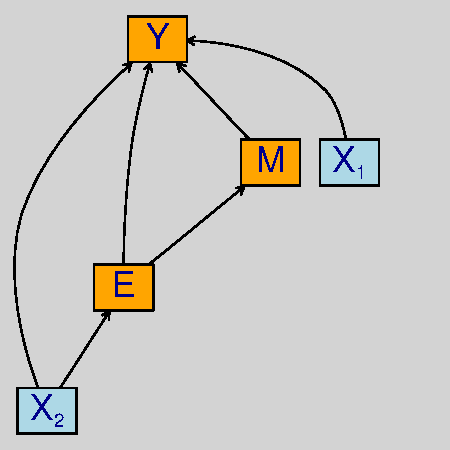
\includegraphics[width=0.7\textwidth]{c:/Users/hpl802/Documents/GitHub/lavaSearch2/vignettes/figures/pathDiagram.pdf}
\caption{\label{fig:pathDiagram}
Path diagram relating the variables Y, E, M, \(X_1\) and \(X_2\)}
\end{figure}}. Doing so we would remove the effect of
\(E\) mediated by \(M\) and therefore bias the estimate of the total
effect (we would only get the direct effect).
\end{itemize}

In the following we will assume that we do not measure any mediator
variable and therefore ignore this type of variable. Also we will call
covariates the variables \(E,X_1,X_2\).

\subsection{Statistical model}
\label{sec:orgd07908d}

We will use a statistical model to relate the observed variables based
a priori assumptions:
\begin{itemize}
\item \textbf{causal assumptions}: saying which variables are related and in
which direction. This can be done by drawing a path diagram similar
to \autoref{fig:pathDiagram}. In simple univariate models it may seems
unnecessary to draw the path diagram since the system of variables is
very simple to visualize. In multivariate model, it is often very
useful to draw it. Some of these assumptions are untestable,
e.g. often we cannot decide whether it is \(E\) that impacts \(Y\)
or whether it is \(Y\) that impacts \(E\) just based on the data.
\item \textbf{modeling assumptions}: specifying the type of relationship between
variables (e.g. linear) and the marginal or joint distribution
(e.g. Gaussian). Often these assumptions can be tested and relaxed
using a more flexible model. While appealing, there are some
drawbacks with using a very flexible model: more data are needed to
get precise estimates and the interpretation of the results is more
complex.
\end{itemize}

A statistical model \(\model\) is set of possible probability
distributions. For instance when we fit a Gaussian linear model for
\(Y_1\) with just an intercept \(\model=\left\{\Gaus[\mu,\sigma^2];\mu
\in \Real, \; \sigma^2 \in \Real^+ \right\}\): \(\model\) is the set
containing all possible univariate normal distributions.

\bigskip

The model parameters are the (non random) variables that enable the
statistical model to "adapt" to different settings. They will be
denoted \(\Theta\). They are the one that are estimated when we fit
the statistical model using the data or that we specify when we
simulate data. In the previous example, we could simulate data
corresponding to a Gaussian linear model using the \texttt{rnorm} function in R:
\lstset{language=r,label= ,caption= ,captionpos=b,numbers=none}
\begin{lstlisting}
rnorm
\end{lstlisting}

\begin{verbatim}
function (n, mean = 0, sd = 1) 
.Call(C_rnorm, n, mean, sd)
<bytecode: 0x000000001d7eb938>
<environment: namespace:stats>
\end{verbatim}

We would need to specify:
\begin{itemize}
\item \(n\) the sample size
\item \(\Theta=(\mu,\sigma^2)\) the model parameters, here \(\mu\) corresponds to \texttt{mean} and \(\sigma\) to \texttt{sd}.
\end{itemize}

\bigskip

The true model parameters are the model parameters that have generated
the observed data. They will be denoted \(\Theta_0\). For instance if
in reality the binding potential is normally distributed with mean 5
and variance \(2^2=4\), then
\(\Theta_0=(\mu_0,\sigma_0^2)=(5,4)\). Then doing our experiment we
observed data such as:
\lstset{language=r,label= ,caption= ,captionpos=b,numbers=none}
\begin{lstlisting}
set.seed(10)
Y_1.XP1 <- rnorm(10, mean = 5, sd = 2)
Y_1.XP1
\end{lstlisting}

\begin{verbatim}
[1] 5.037492 4.631495 2.257339 3.801665 5.589090 5.779589 2.583848 4.272648 1.746655 4.487043
\end{verbatim}

If we were to re-do the experiment we would observe new data but \(\Theta_0\) would not change:
\lstset{language=r,label= ,caption= ,captionpos=b,numbers=none}
\begin{lstlisting}
Y_1.XP2 <- rnorm(10, mean = 5, sd = 2)
Y_1.XP2
\end{lstlisting}

\begin{verbatim}
[1] 7.203559 6.511563 4.523533 6.974889 6.482780 5.178695 3.090112 4.609699 6.851043 5.965957
\end{verbatim}

The estimated parameters are the parameters that we estimate when we
fit the statistical model. They will be denoted \(\Theta_0\). We
usually try to find parameters whose value maximize the chance of
simulating the observed data under the estimated model (maximum
likelihood estimation, MLE). For instance in the first experiment all
values are positive so we would not estimate a negative mean value. In
our example, \(\hat{\mu}\) the MLE of \(\mu\) reduces to the empirical
average and \(\hat{\sigma}^2\) the MLE of \(\sigma^2\) to the
empirical variance:
\lstset{language=r,label= ,caption= ,captionpos=b,numbers=none}
\begin{lstlisting}
Theta_hat.XP1 <- c(mu_hat = mean(Y_1.XP1),
		   sigma2_hat = var(Y_1.XP1))
Theta_hat.XP1
\end{lstlisting}

\begin{verbatim}
  mu_hat sigma2_hat 
4.018686   1.959404
\end{verbatim}

Clearly the estimated coefficients vary across experiments:
\lstset{language=r,label= ,caption= ,captionpos=b,numbers=none}
\begin{lstlisting}
Theta_hat.XP2 <- c(mu_hat = mean(Y_1.XP2),
		   sigma2_hat = var(Y_1.XP2))
Theta_hat.XP2
\end{lstlisting}

\begin{verbatim}
  mu_hat sigma2_hat 
5.739183   1.799311
\end{verbatim}

\subsection{Parameter of interest}
\label{sec:orgf99054a}

The statistical model may contain many parameters, most of them are
often not of interest but are needed to obtain valid estimates
(e.g. account for confounders). In most settings, the parameter of
interest is one (or several) model parameter(s) - or simple
transformation of them. For instance if we are interested in the
average binding potential in the population our parameter of interest
is \(\mu\).

\bigskip

Often, the aim of a study is to obtain the best estimate of the
parameter of interest \(\mu\). Best means:
\begin{itemize}
\item \textbf{unbiased}: if we were able to replicate the study many times,
i.e. get several estimates \(\hat{\mu}_1,\hat{\mu}_2,\ldots,\hat{\mu}_K\), the
average estimate \(<\hat{\mu}>=\frac{\hat{\mu}_1+\hat{\mu}_2+\ldots+\hat{\mu}_K}{K}\) would coincide with the true one \(\mu_0\).
\item \textbf{minimal variance}: if we were able to replicate the study many
times, the variance of the estimates
\(\frac{(\hat{\mu}_1-<\hat{\mu}>)^2+\ldots+(\hat{\mu}_K-<\hat{\mu}>)^2}{K-1}\)
should be as low as possible.
\end{itemize}

There will often be a trade-off between these two objectives. A very
flexible method is more likely to give an unbiased estimate
(e.g. being able to model non-linear relationship) at the price of
greater uncertainty about the estimates. Often we favor unbiasedness
over minimal variance. Indeed, if several studies are published with
the same parameter of interest, one can pool the results to obtain an
estimate with lower variance. Note that we have no guarantee that it
will reduce the bias.

\subsection{Inference}
\label{sec:org624ccae}

In addition to estimate the parameter(s) of interest, we often want to
test hypotheses about the parameter(s) of interest. 

\subsubsection{One parameter}
\label{sec:org6878ca7}

Imagine we fit a univariate linear model relating outcome 1 (\(Y1\))
to exposure 1 (\(E1\)):
\begin{align*}
Y1 = \alpha + \beta E1 + \varepsilon
\end{align*}
where \(\varepsilon\) are the residuals that are assumed to be
 independent and identically distributed (iid) as well as normally
 distributed. Under causal assumptions (mainly no unobserved
 confounder) \(\beta\) denotes the effect of exposure 1, i.e. the
 change in \(Y1\) for each unit increase in \(E1\). In R code we can
 fit the linear model using:
\lstset{language=r,label= ,caption= ,captionpos=b,numbers=none}
\begin{lstlisting}
e.lm <- lm(Y1 ~ E1, data = dtW)
\end{lstlisting}

\begin{verbatim}

Call:
lm(formula = Y1 ~ E1, data = dtW)

Coefficients:
(Intercept)           E1  
   -0.34331     -0.08887
\end{verbatim}

and output the estimated \(\alpha\) and \(\beta\) using \texttt{coef}:
\lstset{language=r,label= ,caption= ,captionpos=b,numbers=none}
\begin{lstlisting}
coef(e.lm)
\end{lstlisting}

\begin{verbatim}
(Intercept)          E1 
-0.34330792 -0.08886769
\end{verbatim}

Imagine we want to test whether there is any association between the
exposure and the exposure. We want to test the null hypothesis:
\begin{align*}
(\Hypothesis[0]) \; \beta = 0
\end{align*}
 Since the parameters are estimated by ML and assuming that the model
is correctly specified, we know that the asymptotic distribution of
the parameter is Gaussian. This means that for large sample size, the
fluctuation of the estimated values follows a normal distribution. For
instance:
\begin{align*}
\hat{\beta} \underset{n \rightarrow \infty}{\sim} \Gaus[\beta,\sigma^2_\beta]
\end{align*}
where \(\sigma^2_\beta\) is the variance of the MLE, i.e. the
incertainty surrounding our estimation of the association. It follows that:
\begin{align}
t_{\beta} = \frac{\hat{\beta}-\beta}{\sigma^2_\beta} \underset{n \rightarrow \infty}{\sim} \Gaus[0,1] \label{eq:uniWald}
\end{align}
So under the null hypothesis of no association between the outcome and
the exposure the statistic \(t_{\beta}\) should follow a standard
normal distribution. Very low or very large values are unlikely to be
observed and would indicate that the null hypothesis does not
hold. This is called a (univariate) Wald test. The result of this
tests can be obtained using the \texttt{summary} method:
\lstset{language=r,label= ,caption= ,captionpos=b,numbers=none}
\begin{lstlisting}
summary(e.lm)$coef
\end{lstlisting}

\begin{verbatim}
               Estimate Std. Error    t value   Pr(>|t|)
(Intercept) -0.34330792  0.1720656 -1.9952158 0.05171268
E1          -0.08886769  0.1787466 -0.4971712 0.62133806
\end{verbatim}

\emph{Note:} in reality R is automatically performing a correction that
improves the control of the type 1 error. Indeed we usually don't know
\(\sigma^2_\beta\) and plugging-in its estimate in equation
\eqref{eq:uniWald} modifies the distribution of \(t_{\beta}\) in small
samples. The correction uses a Student's t distribution instead of a
Gaussian distribution.

\subsubsection{Linear combination of parameters}
\label{sec:org9944b35}

Imagine we now want to test whether the effect of exposure 1 is
different from the effect of exposure 2. We consider the following
univariate linear model:
\begin{align*}
Y1 = \alpha + \beta_1 E1 + \beta_2 E2 + \varepsilon
\end{align*}
where \(\varepsilon\) are assumed to be iid and normally
 distributed. In R code we can fit the linear model using:
\lstset{language=r,label= ,caption= ,captionpos=b,numbers=none}
\begin{lstlisting}
e.lm <- lm(Y1 ~ E1 + E2, data = dtW)
\end{lstlisting}

We want to test the null hypothesis:
\begin{align*}
(\Hypothesis[0]) \; \beta_2 - \beta_1 = 0
\end{align*}
Once more we use that the asymptotic distribution of the parameters is
a normal distribution:
\begin{align*}
\begin{bmatrix}
\hat{\beta}_1 \\ \hat{\beta}_2 \\
\end{bmatrix}
\underset{n \rightarrow \infty}{\sim}
\Gaus \left(\begin{bmatrix}
\hat{\beta}_1 \\ \hat{\beta}_2 \\
\end{bmatrix},
\begin{bmatrix}
\sigma^2_1 & \sigma^2_{12} \\
\sigma^2_{12} & \sigma^2_2 \\
\end{bmatrix}
\right)
\end{align*}
Then \(\beta_1 - \beta_2\) also follows a normal distribution:
\begin{align*}
\hat{\beta}_B - \hat{\beta}_A  \underset{n \rightarrow \infty}{\sim} \Gaus[\beta_B - \beta_A,\sigma^2_B+\sigma^2_A-2\sigma^2_{AB}]
\end{align*}
so:
\begin{align*}
t_{\beta_B-\beta_A} = \frac{\hat{\beta}_B - \hat{\beta}_A - (\beta_B - \beta_A)}{\sigma^2_B+\sigma^2_A-2\sigma^2_{AB}}  \underset{n \rightarrow \infty}{\sim} \Gaus[0,1]
\end{align*}
As before we can compute \(t_{\beta_B-\beta_A}\) under the
 \(\Hypothesis[0]\) and large or low values would be evidence for
 rejecting \(\Hypothesis[0]\). The package \emph{multcomp} provides a
 convenient interface to test linear combinations of parameters. First
 we specify the null hypothesis using the \texttt{glht} method:
\lstset{language=r,label= ,caption= ,captionpos=b,numbers=none}
\begin{lstlisting}
e.glht <- glht(e.lm, linfct = c("E2 - E1 = 0"))
\end{lstlisting}

Then we can use the \texttt{summary} method to obtain perform the test:
\lstset{language=r,label= ,caption= ,captionpos=b,numbers=none}
\begin{lstlisting}
summary(e.glht)
\end{lstlisting}
\begin{verbatim}

	 Simultaneous Tests for General Linear Hypotheses

Fit: lm(formula = Y1 ~ E1 + E2, data = dtW)

Linear Hypotheses:
             Estimate Std. Error t value Pr(>|t|)
E2 - E1 == 0 -0.05015    0.21814   -0.23    0.819
(Adjusted p values reported -- single-step method)
\end{verbatim}

\subsubsection{Linear combination of parameters - using a contrast matrix}
\label{sec:org9d0a31b}

Null hypotheses can be defined using a contrast matrix. If we denote
by:
\begin{align*}
\Theta=[\alpha \; \beta_1 \; \beta_2]
\end{align*}
the vector of parameters, we can define a 1-row contrast matrix:
\begin{align*}
c=[0 \; -1 \; 1]
\end{align*}
such that: 
\begin{align*}
(\Hypothesis[0]) \; c \Theta = \beta_2 - \beta_1 = 0
\end{align*}
Indeed
\begin{align*}
\trans{c} \Theta = 0 * \alpha + -1 * \beta_1 + 1 * \beta_2 = \mu_B - \mu_A
\end{align*}
So in the previous example we could have also defined a contrast
matrix, e.g. using \texttt{createContrast}:
\lstset{language=r,label= ,caption= ,captionpos=b,numbers=none}
\begin{lstlisting}
C <- createContrast(e.lm, par = c("E2 - E1 = 0"),
		    add.variance = FALSE, rowname.rhs = FALSE)
C$contrast
\end{lstlisting}

\begin{verbatim}
          (Intercept) E1 E2
- E1 + E2           0 -1  1
\end{verbatim}

and then call \texttt{glht} using this contrast matrix:
\lstset{language=r,label= ,caption= ,captionpos=b,numbers=none}
\begin{lstlisting}
ebis.glht <- glht(e.lm, linfct = C$contrast)
summary(ebis.glht)
\end{lstlisting}

\begin{verbatim}

	 Simultaneous Tests for General Linear Hypotheses

Fit: lm(formula = Y1 ~ E1 + E2, data = dtW)

Linear Hypotheses:
               Estimate Std. Error t value Pr(>|t|)
- E1 + E2 == 0 -0.05015    0.21814   -0.23    0.819
(Adjusted p values reported -- single-step method)
\end{verbatim}

\subsubsection{Testing simultaneously several combination of parameters}
\label{sec:introMultComp}
When we want to test several hypotheses we can stack the contrast
vector of each hypothesis into the contrast matrix:
\begin{align*}
C = \begin{bmatrix}
0 & 1 & 0 \\
0 & 0 & 1 \\
\end{bmatrix}
\end{align*}
Then \(C \Theta = 0\) is equivalent to:
\begin{align*}
(\Hypothesis[0,I]) \; \beta_1 = 0 \\
(\Hypothesis[0,II]) \; \beta_2 = 0
\end{align*}

For instance we could want to test the null hypothesis that the effect
of both exposures is null:
\lstset{language=r,label= ,caption= ,captionpos=b,numbers=none}
\begin{lstlisting}
C <- createContrast(e.lm, par = c("E1 = 0","E2 = 0"),
		    add.variance = FALSE, rowname.rhs = FALSE)$contrast
C
\end{lstlisting}

\begin{verbatim}
   (Intercept) E1 E2
E1           0  1  0
E2           0  0  1
\end{verbatim}

We can then call \texttt{glht} with this new contrast matrix:
\lstset{language=r,label= ,caption= ,captionpos=b,numbers=none}
\begin{lstlisting}
e.glht <- glht(e.lm, linfct = C)
e.glht
\end{lstlisting}

\begin{verbatim}

	 General Linear Hypotheses

Linear Hypotheses:
        Estimate
E1 == 0  -0.1628
E2 == 0  -0.2130
\end{verbatim}

Since we perform multiple tests, we need to say to the software how to
adjust for multiple comparisons. The \emph{multcomp} package implement several approaches such as:
\begin{itemize}
\item \textbf{no adjustment}:
\end{itemize}
\lstset{language=r,label= ,caption= ,captionpos=b,numbers=none}
\begin{lstlisting}
summary(e.glht, test = adjusted("none"))
\end{lstlisting}

\begin{verbatim}
	 Simultaneous Tests for General Linear Hypotheses

Fit: lm(formula = Y1 ~ E1 + E2, data = dtW)

Linear Hypotheses:
        Estimate Std. Error t value Pr(>|t|)
E1 == 0  -0.1628     0.1905  -0.855    0.397
E2 == 0  -0.2130     0.1925  -1.107    0.274
(Adjusted p values reported -- none method)
\end{verbatim}

\begin{itemize}
\item \textbf{Bonferroni} adjustment (conservative approach)
\end{itemize}
\lstset{language=r,label= ,caption= ,captionpos=b,numbers=none}
\begin{lstlisting}
summary(e.glht, test = adjusted("bonferroni"))
\end{lstlisting}

\begin{verbatim}
	 Simultaneous Tests for General Linear Hypotheses

Fit: lm(formula = Y1 ~ E1 + E2, data = dtW)

Linear Hypotheses:
        Estimate Std. Error t value Pr(>|t|)
E1 == 0  -0.1628     0.1905  -0.855    0.794
E2 == 0  -0.2130     0.1925  -1.107    0.548
(Adjusted p values reported -- bonferroni method)
\end{verbatim}

\begin{itemize}
\item \textbf{single step Dunnett} adjustment (more efficient approach relying on
asymptotic results)
\end{itemize}
\lstset{language=r,label= ,caption= ,captionpos=b,numbers=none}
\begin{lstlisting}
summary(e.glht, test = adjusted("single-step"))
\end{lstlisting}

\begin{verbatim}
	 Simultaneous Tests for General Linear Hypotheses

Fit: lm(formula = Y1 ~ E1 + E2, data = dtW)

Linear Hypotheses:
        Estimate Std. Error t value Pr(>|t|)
E1 == 0  -0.1628     0.1905  -0.855    0.620
E2 == 0  -0.2130     0.1925  -1.107    0.456
(Adjusted p values reported -- single-step method)
\end{verbatim}

\emph{multcomp} also implements approaches that are more powerful than the
single step Dunnett but does not propose the corresponding confidence
intervals (e.g. \texttt{adjusted("free")}). For this reason, they will not be
presented here.

\clearpage

\section{Using a separate model for each outcome}
\label{sec:org9c05834}

In this section, we will model the relationship between each of the
five outcomes and the covariates using a separate linear model:

\begin{align*}
\begin{bmatrix} 
Y_1  &= \alpha_{X_{1}} + \beta_{Y_1,X_0} X_{0} + \beta_{Y_1,X_1} X_{1} + \beta_{Y_1,X_2} X_{2} + \varepsilon_{Y_1} \\
Y_2  &= \alpha_{X_{2}} + \beta_{Y_2,X_0} X_{0} + \beta_{Y_2,X_1} X_{1} + \beta_{Y_2,X_2} X_{2} + \varepsilon_{Y_2} \\
Y_3  &= \alpha_{X_{3}} + \beta_{Y_3,X_0} X_{0} + \beta_{Y_3,X_1} X_{1} + \beta_{Y_3,X_2} X_{2} + \varepsilon_{Y_3} \\
Y_4  &= \alpha_{X_{4}} + \beta_{Y_4,X_0} X_{0} + \beta_{Y_4,X_1} X_{1} + \beta_{Y_4,X_2} X_{2} + \varepsilon_{Y_4} \\
Y_5  &= \alpha_{X_{5}} + \beta_{Y_5,X_0} X_{0} + \beta_{Y_5,X_1} X_{1} + \beta_{Y_5,X_2} X_{2} + \varepsilon_{Y_5} 
\end{bmatrix} 
\end{align*}
where
\(\varepsilon_{1},\varepsilon_{2},\varepsilon_{3},\varepsilon_{4},\varepsilon_{5}\)
are the residual errors. The outcomes are assumed to have zero mean
and finite variance, respectively,
\(\sigma^2_{1},\sigma^2_{2},\sigma^2_{3},\sigma^2_{4},\sigma^2_{5}\). Here
we make no assumption on the correlation structure between the
residuals.


\subsection{Univariate linear regression}
\label{sec:org9d2bcb6}

First, we focus on the first outcome, i.e. the first equation:
\begin{align*}
Y_{1} = \alpha_{X_{1}} + \beta_{Y_1,X_0} X_{0} + \beta_{Y_1,X_1} X_{1} + \beta_{Y_1,X_2} X_{2} + \varepsilon_{Y_1} 
\end{align*}


\subsubsection{Estimation of the model}
\label{sec:org85a3e13}

We can estimate the model parameters
(\(\alpha_{X_{1}},\beta_{Y_1,X_0},\beta_{Y_1,X_1},\beta_{Y_1,X_2},\sigma^2_{Y_1}\))
using \texttt{lm}:
\lstset{language=r,label= ,caption= ,captionpos=b,numbers=none}
\begin{lstlisting}
e.lm <- lm(Y1 ~ E0+E1+E2, data = dtW)
\end{lstlisting}

The estimate model parameters
(\(\hat{\alpha}_{X_{1}},\hat{\beta}_{Y_1,X_0},\hat{\beta}_{Y_1,X_1},\hat{\beta}_{Y_1,X_2},\hat{\sigma}^2_{Y_1}\))
can be output using \texttt{summary}:
\lstset{language=r,label= ,caption= ,captionpos=b,numbers=none}
\begin{lstlisting}
summary(e.lm)$coef
\end{lstlisting}

\begin{verbatim}
               Estimate Std. Error     t value   Pr(>|t|)
(Intercept) -0.38648123  0.1783576 -2.16689009 0.03545788
E0          -0.01097614  0.1799681 -0.06098939 0.95163188
E1          -0.16366671  0.1929686 -0.84815191 0.40074529
E2          -0.21367875  0.1948854 -1.09643293 0.27859637
\end{verbatim}

or \texttt{coef}:
\lstset{language=r,label= ,caption= ,captionpos=b,numbers=none}
\begin{lstlisting}
coef(e.lm)
\end{lstlisting}

\begin{verbatim}
(Intercept)          E0          E1          E2 
-0.38648123 -0.01097614 -0.16366671 -0.21367875
\end{verbatim}

Confidence intervals can be obtained with the \texttt{confint} method:
\lstset{language=r,label= ,caption= ,captionpos=b,numbers=none}
\begin{lstlisting}
confint(e.lm)
\end{lstlisting}

\begin{verbatim}
                 2.5 %      97.5 %
(Intercept) -0.7454964 -0.02746608
E0          -0.3732331  0.35128081
E1          -0.5520924  0.22475899
E2          -0.6059627  0.17860517
\end{verbatim}

\subsubsection{Fitted values}
\label{sec:org80fb794}

A fitted value, denoted \(\hat{Y}\), is the expected outcome value
estimated by the model. When there are covariates included in the
model (e.g. \(X_{0}\), \(X_{1}\), \(X_{2}\)), the fitted value depends
on the value of the covariates. In a linear model, the fitted values
can be computed using:
\begin{align*}
\hat{Y} = \hat{\alpha}_{X_{1}} + \hat{\beta}_{Y_1,X_0} X_{0} + \hat{\beta}_{Y_1,X_1} X_{1} + \hat{\beta}_{Y_1,X_2} X_{2}
\end{align*}
This can be done in R using the \texttt{fitted} method:
\lstset{language=r,label= ,caption= ,captionpos=b,numbers=none}
\begin{lstlisting}
dtW$fit.lm <- fitted(e.lm)
dtW$fit.lm[1]
\end{lstlisting}

\begin{verbatim}
[1] -0.1738311
\end{verbatim}

One can also compute them using:
\lstset{language=r,label= ,caption= ,captionpos=b,numbers=none}
\begin{lstlisting}
coef(e.lm)["(Intercept)"] + coef(e.lm)["E0"] * dtW$E0[1] + coef(e.lm)["E1"] * dtW$E1[1] + coef(e.lm)["E2"] * dtW$E2[1]
\end{lstlisting}

\begin{verbatim}
(Intercept) 
 -0.1738311
\end{verbatim}

\subsubsection{Diagnostics}
\label{sec:diagLM}
Inference using a univariate linear model rely on several assumptions:
\begin{itemize}
\item residuals independent and identically distributed (iid).
\item residuals normally distributed.
\item correct specification of the linear predictor, e.g. linearity of the effect, no interaction.
\item no unobserved confounders (this is usually an untestable
assumption).
\end{itemize}
Moreover, explanatory variables that are very correlated may lead to
instable results.

\bigskip

By default R provides a graphical display that enables to check
several of these assumptions:
\lstset{language=r,label= ,caption= ,captionpos=b,numbers=none}
\begin{lstlisting}
par(mfrow = c(2,2))
plot(e.lm)
\end{lstlisting}



\begin{center}
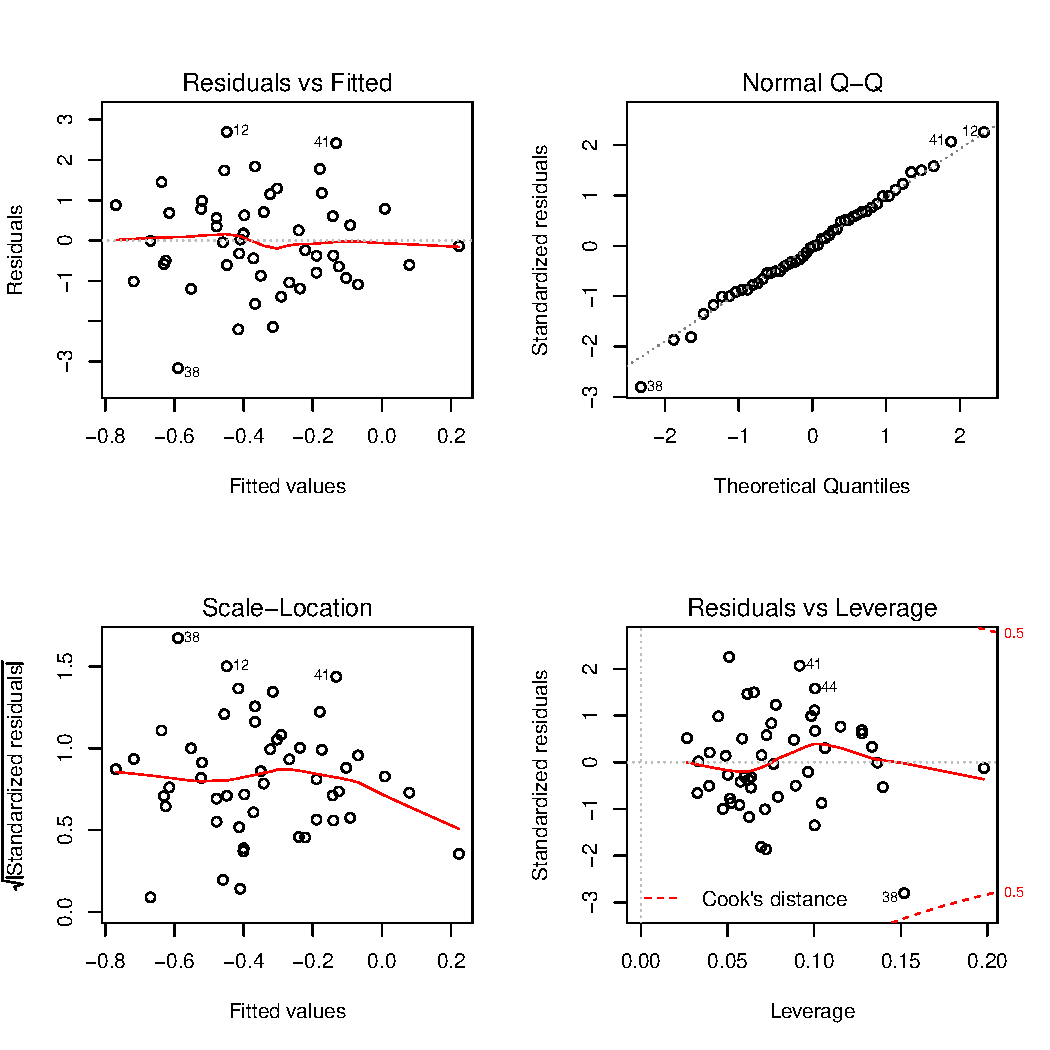
\includegraphics[width=.9\linewidth]{c:/Users/hpl802/Documents/GitHub/lavaSearch2/vignettes/figures/diag-lm.pdf}
\end{center}

The top left plot is useful to detect a misspecification of the linear
predictor (e.g. a U shape would indicate a missing quadratic
effect). The top right plot enable to check the normality of the
residuals, we will describe a more informative qqplot below. The
bottom left can be used to detect heteroschedasticity (e.g. a trumpet
shape) and the bottom right plot can be used to identify observation
that have a huge influence on the fitted values.

\bigskip

The \textbf{qqtest} package provides a more readable qqplot. To use it, we
first need to extract the residuals. This can be achieved using the
\texttt{residuals} method:
\lstset{language=r,label= ,caption= ,captionpos=b,numbers=none}
\begin{lstlisting}
dtW$resid.lm <- residuals(e.lm, type = "response")
\end{lstlisting}

The \texttt{type} argument indicates the type of residuals we want to
extract. Raw residuals are \(\hat{\varepsilon} = Y-\hat{Y}\), i.e. the observed minus the
fitted values. In models more complex than a univariate linear
regression, the raw residuals may not be iid. This makes it difficult
to assess the validity of the assumptions. This is why we usually
display diagnostics for normalized residuals that, if the assumptions
of the model are correct, should follow a standard normal
distribution. For instance in the case of a univariate linear model,
we can use the Pearson residuals:

\begin{align*}
\hat{\varepsilon}^{Pearson} = \frac{Y-\hat{Y}}{\sqrt{\Var[\hat{Y}]}} \sim \Gaus[0,1]
\end{align*}
In R:
\lstset{language=r,label= ,caption= ,captionpos=b,numbers=none}
\begin{lstlisting}
sd.resid <- sigma(e.lm)*sqrt(1-lm.influence(e.lm, do.coef = FALSE)$hat)
dtW$resid.norm.lm <- dtW$resid.lm/sd.resid
\end{lstlisting}

We can then obtain the qqplot using the \texttt{qqtest} function:
\lstset{language=r,label= ,caption= ,captionpos=b,numbers=none}
\begin{lstlisting}
qqtest(dtW$resid.norm.lm)
\end{lstlisting}

\begin{center}
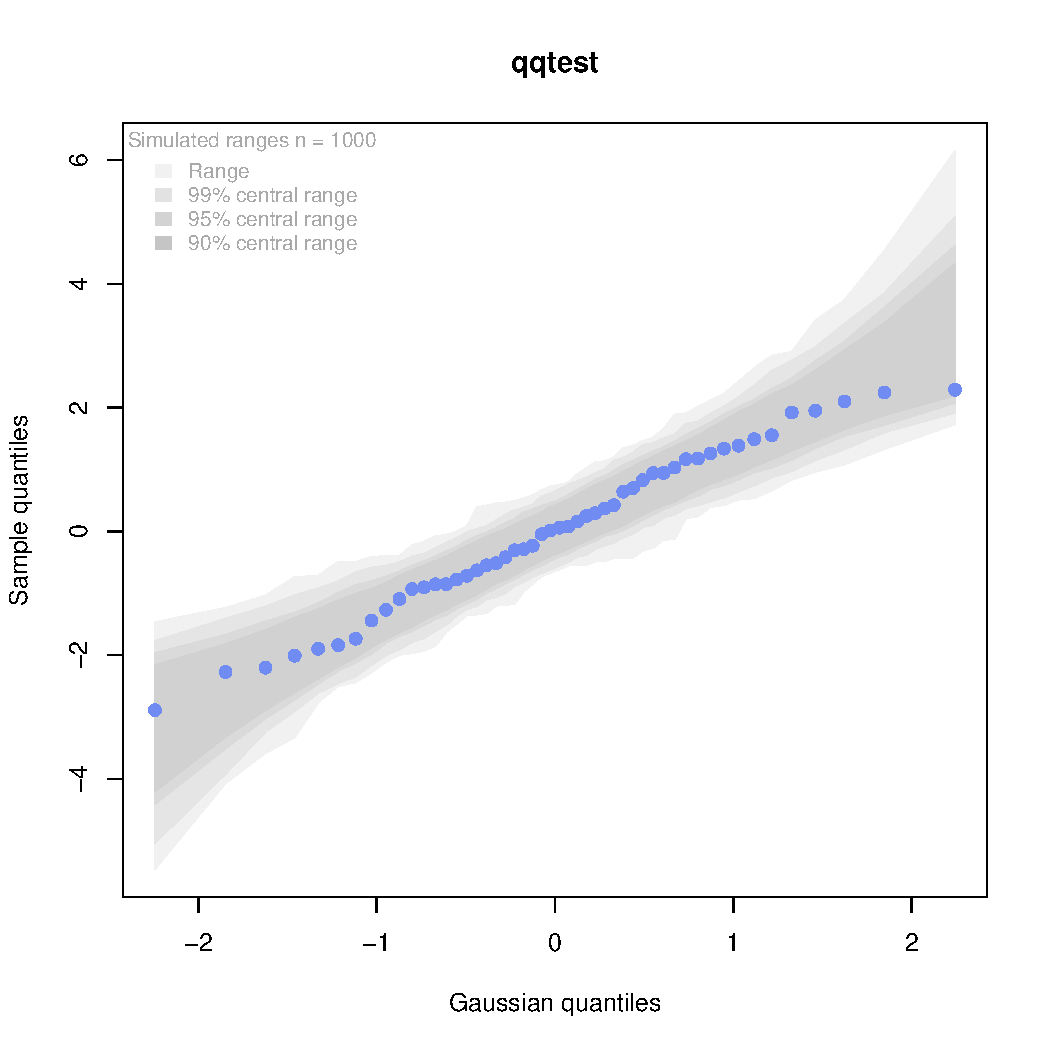
\includegraphics[width=.9\linewidth]{c:/Users/hpl802/Documents/Projects/Neuropharm/WP1/figures/qqplot-lm.pdf}
\end{center}

The shaded area indicates where, if the normality assumption was
correct, we would expect to observe the points. Alternatively, an
histogram of the residuals can be used to assess the normality of the
residuals:
\lstset{language=r,label= ,caption= ,captionpos=b,numbers=none}
\begin{lstlisting}
hist(dtW$resid.lm, prob=TRUE)
curve(dnorm(x, mean=0, sd=1), add=TRUE, col = "red")
\end{lstlisting}

\begin{center}
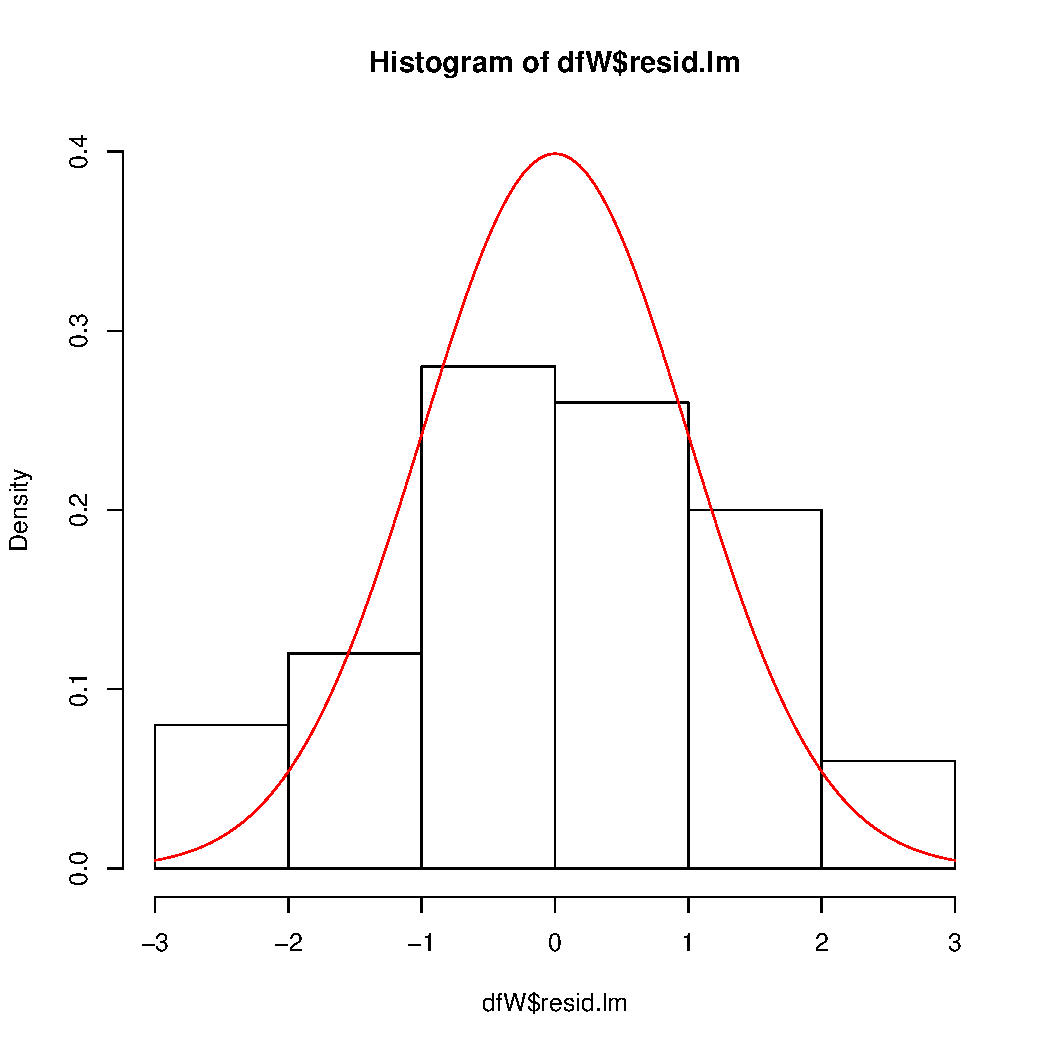
\includegraphics[width=.9\linewidth]{c:/Users/hpl802/Documents/GitHub/lavaSearch2/vignettes/figures/hist-lm.pdf}
\end{center}

Statistical tests can also be used to assess deviation from normality:
\lstset{language=r,label= ,caption= ,captionpos=b,numbers=none}
\begin{lstlisting}
shapiro.test(dtW$resid.lm)
\end{lstlisting}

\begin{verbatim}

	Shapiro-Wilk normality test

data:  dtW$resid.lm
W = 0.99284, p-value = 0.9899
\end{verbatim}
Here the null hypothesis is that the residuals follow a normal
distribution.

\bigskip

The \texttt{influence} method can be used to output what is the impact of
each observation on each estimated parameter:
\lstset{language=r,label= ,caption= ,captionpos=b,numbers=none}
\begin{lstlisting}
head(influence(e.lm)$coefficient)
\end{lstlisting}

\begin{verbatim}
   (Intercept)           E0           E1           E2
1  0.023113692 -0.014298361 -0.026854342 -0.014861558
2  0.013331967 -0.005188019  0.005660896  0.001314494
3  0.009519952  0.011090606 -0.004793503  0.010612459
4  0.012117058  0.036241781  0.011800078 -0.006132586
5 -0.015026578 -0.007331698  0.020875655  0.021232975
6  0.008123937  0.012157294 -0.003719040 -0.042740303
\end{verbatim}

\bigskip

A statistical test can also be used to assess whether there is
evidence for a more complex functional form for the linear predictor:
\lstset{language=r,label= ,caption= ,captionpos=b,numbers=none}
\begin{lstlisting}
cumres(e.lm)
\end{lstlisting}

\begin{verbatim}
Kolmogorov-Smirnov-test: p-value=0.749
Cramer von Mises-test: p-value=0.764
Based on 1000 realizations. Cumulated residuals ordered by predicted-variable.
---
Kolmogorov-Smirnov-test: p-value=0.278
Cramer von Mises-test: p-value=0.27
Based on 1000 realizations. Cumulated residuals ordered by E0-variable.
---
Kolmogorov-Smirnov-test: p-value=0.413
Cramer von Mises-test: p-value=0.529
Based on 1000 realizations. Cumulated residuals ordered by E1-variable.
---
Kolmogorov-Smirnov-test: p-value=0.436
Cramer von Mises-test: p-value=0.762
Based on 1000 realizations. Cumulated residuals ordered by E2-variable.
---
\end{verbatim}

\bigskip

Finally, an excessive correlation among the explanatory variables can
be detected using the VIF (variance inflation factor):
\lstset{language=r,label= ,caption= ,captionpos=b,numbers=none}
\begin{lstlisting}
vif(e.lm)
\end{lstlisting}

\begin{verbatim}
      E0       E1       E2 
1.006096 1.146089 1.144345
\end{verbatim}
Values higher than 5 are (arbitrarily) considered as high.

\subsection{Multiple linear regressions}
\label{sec:orgd0f8d3b}


We now estimate all the 5 models and store them into a list:
\lstset{language=r,label= ,caption= ,captionpos=b,numbers=none}
\begin{lstlisting}
ls.lm <- list(Y1 = lm(Y1 ~ E0+E1+E2, data = dtW),
	      Y2 = lm(Y2 ~ E0+E1+E2, data = dtW),
	      Y3 = lm(Y3 ~ E0+E1+E2, data = dtW),
	      Y4 = lm(Y4 ~ E0+E1+E2, data = dtW),
	      Y5 = lm(Y5 ~ E0+E1+E2, data = dtW)
	      )
\end{lstlisting}

The next step would be to check the hypotheses relative to each of the
models (see section \ref{sec:diagLM}). To perform inference in this setting
we first need to define our null hypothesis or null hypotheses. Let
imagine that we want to test the effect of the exposure E0 and say
whether any outcome is related to the exposure. We first define a
contrast matrix:

\lstset{language=r,label= ,caption= ,captionpos=b,numbers=none}
\begin{lstlisting}
resC <- createContrast(ls.lm, var.test = "E1", add.variance = TRUE)
\end{lstlisting}

Since we consider separate model, we will use the element \texttt{mlf} in the
output of \texttt{createContrast}:
\lstset{language=r,label= ,caption= ,captionpos=b,numbers=none}
\begin{lstlisting}
resC$mlf
\end{lstlisting}
\begin{verbatim}
$Y1
   (Intercept) E0 E1 E2 sigma2
E1           0  0  1  0      0

$Y2
   (Intercept) E0 E1 E2 sigma2
E1           0  0  1  0      0

$Y3
   (Intercept) E0 E1 E2 sigma2
E1           0  0  1  0      0

$Y4
   (Intercept) E0 E1 E2 sigma2
E1           0  0  1  0      0

$Y5
   (Intercept) E0 E1 E2 sigma2
E1           0  0  1  0      0

attr(,"class")
[1] "mlf"
\end{verbatim}

is the left hand side of the null hypothesis and:
\lstset{language=r,label= ,caption= ,captionpos=b,numbers=none}
\begin{lstlisting}
resC$null
\end{lstlisting}

\begin{verbatim}
Y1: E0 Y2: E0 Y3: E0 Y4: E0 Y5: E0 
     0      0      0      0      0
\end{verbatim}

is the right hand side of the null hypothesis. We can now call
\texttt{glht2}. To do so we first need to convert the list into a \texttt{mmm} object:
\lstset{language=r,label= ,caption= ,captionpos=b,numbers=none}
\begin{lstlisting}
class(ls.lm) <- "mmm"
e.glht_lm <- glht2(ls.lm, linfct = resC$contrast, rhs = resC$null)
e.glht_lm
\end{lstlisting}

\begin{verbatim}
	 General Linear Hypotheses

Linear Hypotheses:
            Estimate
Y1: E1 == 0 -0.16367
Y2: E1 == 0 -0.09144
Y3: E1 == 0 -0.22923
Y4: E1 == 0  0.02596
Y5: E1 == 0 -0.73954
\end{verbatim}

We can now correct for multiple comparisons using the methods
presented in section \ref{sec:introMultComp}:
\lstset{language=r,label= ,caption= ,captionpos=b,numbers=none}
\begin{lstlisting}
summary(e.glht_lm, test = adjusted("single-step"))
\end{lstlisting}

\begin{verbatim}
	 Simultaneous Tests for General Linear Hypotheses

Linear Hypotheses:
            Estimate Std. Error t value Pr(>|t|)
Y1: E1 == 0 -0.16367    0.19297  -0.848    0.766
Y2: E1 == 0 -0.09144    0.40563  -0.225    0.998
Y3: E1 == 0 -0.22923    0.44975  -0.510    0.949
Y4: E1 == 0  0.02596    0.18949   0.137    1.000
Y5: E1 == 0 -0.73954    0.45807  -1.614    0.284
(Adjusted p values reported -- single-step method)
\end{verbatim}

When all the linear model have the same number of degrees of freedom,
the unadjusted p-values of this procedure will match the p-values of
each model. Otherwise an approximation is made and the results may
differ slightly, especially if the sample size is small. Confidence
intervals can be obtained using the \texttt{confint} function:
\lstset{language=r,label= ,caption= ,captionpos=b,numbers=none}
\begin{lstlisting}
confint(e.glht_lm)
\end{lstlisting}

\begin{verbatim}
	 Simultaneous Confidence Intervals

Fit: NULL

Quantile = 2.4946
95% family-wise confidence level
 

Linear Hypotheses:
            Estimate lwr      upr     
Y1: E1 == 0 -0.16367 -0.64505  0.31772
Y2: E1 == 0 -0.09144 -1.10335  0.92046
Y3: E1 == 0 -0.22923 -1.35119  0.89272
Y4: E1 == 0  0.02596 -0.44675  0.49868
Y5: E1 == 0 -0.73954 -1.88226  0.40318
\end{verbatim}
Note that the \texttt{confint} function output confidence intervals using
the (single step) Dunnett correction.

\subsection{Power and type 1 error of the procedure}
\label{sec:orga77729f}

See appendix \ref{appendix:massUnivariate}

\clearpage

\section{References}
\label{sec:org4adb0cb}
\bibliographystyle{apalike}
\bibliography{bibliography}

\clearpage

\appendix

\section{Power and type 1 error}
\label{sec:orgc6bd93e}

\subsection{Multiple linear regression: no adjustment vs. Bonferroni vs. Dunnett}
\label{appendix:massUnivariate}
Fonction replicating the analysis for a given sample size:
\lstset{language=r,label= ,caption= ,captionpos=b,numbers=none}
\begin{lstlisting}
warper_type1power <- function(n.sample){

    ## simulate data
    iDf <- lava::sim(m.sim, n = n.sample, latent = FALSE)

    ## fit model
    iLs <- list(Y1 = lm(Y1 ~ E0+E1+E2, data = iDf),
		Y2 = lm(Y2 ~ E0+E1+E2, data = iDf),
		Y3 = lm(Y3 ~ E0+E1+E2, data = iDf),
		Y4 = lm(Y4 ~ E0+E1+E2, data = iDf),
		Y5 = lm(Y5 ~ E0+E1+E2, data = iDf)
		)
    class(iLs) <- "mmm"

    ## type 1 error
    iC.E0 <- createContrast(iLs, var.test = "E0", add.variance = TRUE)
    iGlht.E0 <- glht2(iLs, linfct = iC.E0$contrast, rhs = iC.E0$null)

    ## power
    iC.E1 <- createContrast(iLs, var.test = "E1", add.variance = TRUE)
    iGlht.E1 <- glht2(iLs, linfct = iC.E1$contrast, rhs = iC.E1$null)

    ## export
    vec.minP <- c("type1.none" = min(summary(iGlht.E0, test = adjusted("none"))$test$pvalues),
		  "type1.bonferroni" = min(summary(iGlht.E0, test = adjusted("bonferroni"))$test$pvalues),
		  "type1.dunnett" = min(summary(iGlht.E0, test = adjusted("single-step"))$test$pvalues),
		  "power.none" = min(summary(iGlht.E1, test = adjusted("none"))$test$pvalues),
		  "power.bonferroni" = min(summary(iGlht.E1, test = adjusted("bonferroni"))$test$pvalues),
		  "power.dunnett" = min(summary(iGlht.E1, test = adjusted("single-step"))$test$pvalues))
    return(vec.minP)
}
\end{lstlisting}

Perform simulation study:
\lstset{language=r,label= ,caption= ,captionpos=b,numbers=none}
\begin{lstlisting}
set.seed(10)
n.cpus <- 4
n.sim <- 1e3

cl <- snow::makeSOCKcluster(n.cpus)
doSNOW::registerDoSNOW(cl)

pb <- txtProgressBar(max = n.sim, style=3)
opts <- list(progress = function(n) setTxtProgressBar(pb, n))

ls.res <- foreach::`%dopar%`(
		       foreach::foreach(i=1:n.sim,
					.options.snow=opts,
					.packages = c("multcomp","lavaSearch2")), {
					    warper_type1power(50)
					})

parallel::stopCluster(cl)
M.p <- Reduce(rbind,ls.res)
\end{lstlisting}

Type 1 error:
\lstset{language=r,label= ,caption= ,captionpos=b,numbers=none}
\begin{lstlisting}
colMeans(M.p[,1:3]<=0.05)
\end{lstlisting}

\begin{verbatim}
type1.none type1.bonferroni    type1.dunnett 
     0.165            0.034            0.057
\end{verbatim}

Power:
\lstset{language=r,label= ,caption= ,captionpos=b,numbers=none}
\begin{lstlisting}
colMeans(M.p[,4:6]<=0.05)
\end{lstlisting}

\begin{verbatim}
power.none power.bonferroni    power.dunnett 
     0.381            0.137            0.178
\end{verbatim}

\clearpage
\end{document}